\documentclass[10pt]{article}
\usepackage[polish]{babel}
\usepackage[utf8]{inputenc}
\usepackage[T1]{fontenc}
\usepackage{amsmath}
\usepackage{amsfonts}
\usepackage{amssymb}
\usepackage[version=4]{mhchem}
\usepackage{stmaryrd}
\usepackage{graphicx}
\usepackage[export]{adjustbox}
\graphicspath{ {./images/} }

\title{LIGA MATEMATYCZNA \\
 im. Zdzisława Matuskiego \\
 FINAE \\
 10 kwietnia 2013 SZKOŁA PODSTAWOWA }

\author{}
\date{}


\begin{document}
\maketitle
\section*{ZADANIE 1.}
Kwadrat \(A B C D\) podzielono na mniejsze kwadraty tak, jak na rysunku. Ile i jakich kwadratów trzeba zamalować, aby powierzchnia zamalowana stanowiła piątą część powierzchni kwadratu \(A B C D\) ? Kwadratów nie można dzielić na mniejsze części.\\
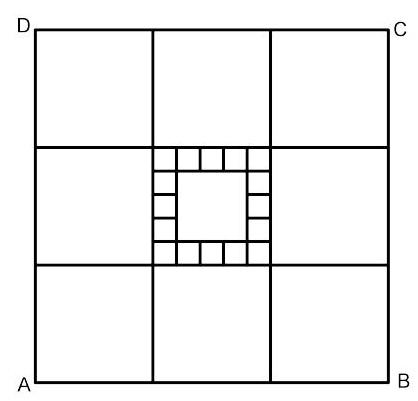
\includegraphics[max width=\textwidth, center]{2024_11_21_8651a206313a84caad96g-1}

\section*{ZADANIE 2.}
Wyznacz cztery różne liczby naturalne parzyste, których iloczyn jest równy 8880.

\section*{ZADANIE 3.}
Dany jest kwadrat \(A B C D\) oraz trójkąt równoboczny \(A B E\), gdzie bok \(A B\) jest wspólny dla obu figur. Wyznacz miarę kąta \(D E C\). Rozważ wszystkie przypadki położenia punktu \(E\).

\section*{ZADANIE 4.}
Liczba uczniów pewnej szkoły podstawowej jest zawarta między 500 a 1000. Gdy grupujemy ich po 18 lub po 20, lub po 24 , to za każdym razem pozostaje 9 uczniów. Ilu uczniów uczęszcza do tej szkoły?

\section*{ZADANIE 5.}
W dwóch workach było 216 kg mąki. Jeśli z pierwszego worka przesypiemy do drugiego 93 kg , a następnie z drugiego worka przesypiemy do pierwszego tyle, aby jego zawartość podwoiła się, to w obu workach będzie tyle samo mąki. Ile kilogramów mąki było w każdym worku na początku?


\end{document}